\documentclass{article}
\usepackage{ae,aecompl}
\usepackage{todonotes}
\usepackage{chngcntr}
\usepackage{tikz-cd}
\usepackage{graphicx}
\graphicspath{ {./images/}}
\usepackage[all,cmtip]{xy}
\usepackage{amsmath, amscd}
\usepackage{amsthm}
\usepackage{amssymb}
\usepackage{amsfonts}
\usepackage{bm}
\usepackage{qsymbols}
\usepackage{latexsym}
\usepackage{mathrsfs}
\usepackage{mathtools}
\usepackage{cite}
\usepackage{color}
\usepackage{url}
\usepackage{enumerate}
\usepackage{verbatim}
\usepackage[draft=false, colorlinks=true]{hyperref}
\usepackage{pdfpages}
\usepackage[margin=1.2in]{geometry}
\usepackage{IEEEtrantools}

\usepackage{fancyhdr}


\usepackage[nameinlink]{cleveref}


\DeclareMathOperator*{\ac}{accept}
\DeclareMathOperator*{\amax}{argmax}
\DeclareMathOperator*{\amin}{argmin}
\DeclareMathOperator*{\Aut}{Aut}
\newcommand {\al}{{\alpha}}
\newcommand {\abs}[1]{{\left\lvert#1\right\rvert}}
\newcommand {\A}{{\mathcal{A}}}
\newcommand {\AM}{{\mathrm{AM}}}
\newcommand {\AMp}{{\AM_{p}^{X}\!(\Ri_\w)}}
\newcommand {\B}{{\mathcal{B}}}
\DeclareMathOperator*{\Be}{Bern}
\newcommand {\Br}{{\dot{B}}}
\newcommand {\Ba}{{\mathfrak{B}}}
\newcommand {\C}{{\mathbb C}}
\newcommand {\ce}{\mathrm{c}}
\newcommand {\Ce}{\mathrm{C}}
\newcommand {\Cc}{\mathrm{C_{c}}}
\newcommand {\Ccinf}{\mathrm{C_{c}^{\infty}}}
\DeclareMathOperator{\cov}{Cov}
\DeclareMathOperator{\DEV}{DEV}
\newcommand {\Di}{{\mathbb D}}
\newcommand {\dom}{\mathrm{dom}}
\newcommand{\dist}{\stackrel{\mathrm{dist}}{=}}
\newcommand {\ud}{\mathrm{d}}
\newcommand {\ue}{\mathrm{e}}
\newcommand {\eps}{\varepsilon}
\newcommand {\veps}{\varepsilon}
\newcommand {\vrho}{{\varrho}}
\newcommand {\E}{{\mathbb{E}}}
\newcommand {\Ec}{{\mathcal{E}}}
\newcommand {\Ell}{L}
\newcommand {\Ellp}{{L_{p}[0,1]}}
\newcommand {\Ellpprime}{{L_{p'}([0,1])}}
\newcommand {\Ellq}{{L_{q}([0,1])}}
\newcommand {\Ellqprime}{{L_{q'}([0,1])}}
\newcommand {\Ellr}{L^{r}}
\newcommand {\Ellone}{{L_{1}([0,1])}}
\newcommand{\Elltwo}{{L_{2}([0,1])}}
\newcommand{\Ellinfty}{L^{\infty}}
\newcommand{\Ellinftyc}{L_{\mathrm{c}}^{\infty}}
\newcommand{\exb}[1]{\exp\left\{#1\right\}}
\DeclareMathOperator*{\Ext}{Ext}
\newcommand{\F}{{\mathcal{F}}}
\newcommand{\Fe}{{\mathbb{F}}}
\newcommand{\G}{{\mathcal{G}}}
\newcommand{\HF}{\mathcal{H}_{\text{FIO}}^{1}(\Rd)}
\newcommand{\Hr}{H}
\newcommand{\HT}{\mathcal{H}}
\newcommand{\ui}{\mathrm{i}}
\newcommand{\I}{{I}}
\newcommand{\J}{{\mathcal{J}}}
\newcommand{\id}{{\mathrm{id}}}
\newcommand{\iid}{\stackrel{\mathclap{\normalfont\mbox{iid}}}{\sim}}
\newcommand{\im}{{\text{im }}}
\newcommand{\ind}{{\perp\!\!\!\perp}}
\DeclareMathOperator*{\Int}{int}
\newcommand{\intx}{{\overline{\int_{X}}}}
\newcommand{\inte}{{\overline{\int_{\E}}}}
\newcommand{\la}{\lambda}
\newcommand{\rb}{\rangle}
\newcommand{\lb}{{\langle}}
\newcommand{\La}{\Lambda}
\newcommand{\calL}{{\mathcal{L}}}
\newcommand{\lp}{{\mathcal{L}}^{p}}
\newcommand{\lpo}{{\overline{\mathcal{L}}^{p}\!}}
\newcommand{\Lpo}{{\overline{\Ell}^{p}\!}}
\newcommand{\M}{{\mathbf{M}}}
\newcommand{\Ma}{{\mathcal{M}}}
\newcommand{\N}{{{\mathbb N}}}
\newcommand{\Na}{{{\mathcal{N}}}}
\newcommand{\norm}[1]{\left\|#1\right\|}
\newcommand{\normm}[1]{{\left\vert\kern-0.25ex\left\vert\kern-0.25ex\left\vert #1 
    \right\vert\kern-0.25ex\right\vert\kern-0.25ex\right\vert}}
\newcommand{\Om}{{{\Omega}}}
\newcommand{\one}{{{\bf 1}}}
\newcommand{\pic}{\text{Pic }}
\newcommand{\ph}{{\varphi}}
\newcommand{\Pa}{{\mathbb{P}}}
\newcommand{\Po}{{\mathcal{P}}}
\newcommand{\Q}{{\mathbb{Q}}}
\newcommand{\R}{{\mathbb R}}
\newcommand{\Rd}{{\mathbb{R}^{d}}}
\DeclareMathOperator{\rej}{reject }
\newcommand{\Rn}{{\mathbb{R}^{n}}}
\newcommand{\cR}{{\mathcal{R}}}
\newcommand{\Rad}{{\mathrm{Rad}}}
\newcommand{\ran}{{\mathrm{ran}}}
\newcommand{\Ri}{{\mathrm{R}}}
\newcommand{\supp}{{\mathrm{supp}}}
\newcommand{\Se}{\mathrm{S}}
\newcommand{\Sp}{S^{*}(\Rn)}
\newcommand{\St}{{\mathrm{St}}}
\newcommand{\Sw}{\mathcal{S}}
\newcommand{\T}{{\mathcal{T}}}
\newcommand{\ta}{{\theta}}
\newcommand{\Ta}{{\Theta}}
\newcommand{\topp}{\stackrel{p}{\to}}
\newcommand{\todd}{\stackrel{d}{\to}}
\newcommand{\toL}[1]{\stackrel{L^{#1}}{\to}} 
\newcommand{\toas}{\stackrel{a.s.}{\to}}
\DeclareMathOperator{\V}{Var}
\newcommand {\w}{{\omega}}
\newcommand {\W}{{\mathrm{W}}}
\newcommand {\Wnp}{\text{$\mathrm{W}$\textsuperscript{$n,\!p$}}}
\newcommand {\Wnpeq}{\text{$\mathrm{W}$\textsuperscript{$n\!,\!p$}}}
\newcommand {\Wonep}{\text{$\mathrm{W}$\textsuperscript{$1,\!p$}}}
\newcommand {\Wonepeq}{\text{$\mathrm{W}$\textsuperscript{$1\!,\!p$}}}
\newcommand {\X}{{\mathcal{X}}}
\newcommand {\Z}{{{\mathbb Z}}}
\newcommand {\Za}{{\mathcal{Z}}}
\newcommand {\Zd}{{\Z[\sqrt{d}]}}
\newcommand {\vanish}[1]{\relax}

\newcommand {\wh}{\widehat}
\newcommand {\wt}{\widetilde}
\newcommand {\red}{\color{red}}

% Distributions
\newcommand{\normal}{\mathsf{N}}
\newcommand{\poi}{\mathsf{Poisson}}
\newcommand{\bern}{\mathsf{Bernoulli}}
\newcommand{\bin}{\mathsf{Binomal}}
\newcommand{\multi}{\mathsf{Multinomial}}
\newcommand{\Exp}{\mathsf{Exp}}



% put your command and environment definitions here




% some theorem environments
% remove "[theorem]" if you do not want them to use the same number sequence


  \newtheorem{thrm}{Theorem}
  \newtheorem{lemma}{Lemma}
  \newtheorem{prop}{Proposition}
  \newtheorem{cor}{Corollary}

  \newtheorem{conj}{Conjecture}
  \renewcommand{\theconj}{\Alph{conj}}  % numbered A, B, C etc

  \theoremstyle{definition}
  \newtheorem{defn}{Definition}
  \newtheorem{ex}{Example}
  \newtheorem{exs}{Examples}
  \newtheorem{question}{Question}
  \newtheorem{remark}{Remark}
  \newtheorem{notn}{Notation}
  \newtheorem{exer}{Exercise}




\title{STATS305A - Lecture 4}
\author{John Duchi\\ Scribed by Michael Howes}
\date{09/30/21}

\pagestyle{fancy}
\fancyhf{}
\rhead{STATS305A - Lecture 4}
\lhead{09/30/21}

\begin{document}
\maketitle
\tableofcontents

\section{Anouncements}
HW1 has been posted on the course webpage. An additional question will be added. The extra question will relate to our first Etude.

\section{Distributions}
\subsection{Recap}
We write $X\sim \Na(\mu,\Sigma)$ is $X \in \R^d$ has a density
\[f(x) = \frac{1}{(2\pi)^{d/2}\det(\Sigma)^{1/2}}\exp\left(-\frac{1}{2}(x-\mu)^T\Sigma^{-1}(x-\mu)\right). \]
We will say $X$ has a normal or Gaussian distribution with mean $\mu$ and covariance $\Sigma$. We have the following magical properties

\begin{itemize}
    \item A normal distribution is determined by its first and second moments.
    \item If $Z \sim \Na(\mu, \Sigma)$, then $Az+b$ is also Gaussian.
    \item If 
    \[\begin{bmatrix}
        X\\Y
    \end{bmatrix}\sim N\left(\begin{bmatrix}
        \mu_1\\ \mu_2
    \end{bmatrix}, \begin{bmatrix}
        \Sigma_{11}&\Sigma_{12}\\
        \Sigma_{21}&\Sigma_{22}
    \end{bmatrix}\right), \]
    then $X \ind Y$ ($X$ is independent of $Y$) if and only if $\Sigma_{12}=0$. (Note that $\Sigma_{21}=\Sigma_{21}^T$ so we have $\Sigma_{21}=0 \iff \Sigma_{12}=0$).
\end{itemize}

\subsection{Chi-squared distributions}
If $Z_i \iid \Na(0,1)$, then 
\[S^2 = \sum_{i=1}^n Z_i^2, \]
has a $\chi_n^2$-distribution. That is $S^2$ has a chi-squared distribution with $n$ degrees of freedom (d.o.f).
\begin{ex}
    [Quadratic forms of Gaussians] If $X \sim \Na(\mu, \Sigma)$ with $\Sigma \succ 0$ and $X \in \R^n$, then we have $S^2 = (X-\mu)^T\Sigma^{-1}(X-\mu) \sim \chi^2_n$.
    \begin{proof}
     Note that $X-\mu \sim N(0,\Sigma)$ and $Z = \Sigma^{-1/2}(X-\mu) \sim N(0,I)$. Thus
     \begin{IEEEeqnarray*}{rCl+x+}
        (X-\mu)^T\Sigma^{-1}(X-\mu)&=&(\Sigma^{-1/2}(X-\mu))^T(\Sigma^{-1/2}(X-\mu))\\
        &=&Z^TZ\\
        &=&\norm{Z}_2^2\\
        &\sim& \chi^2_n.&\qedhere
     \end{IEEEeqnarray*}
    \end{proof}
\end{ex}
\subsection{Projections}

A matrix $\Pi \in \R^{n \times n}$ is a \emph{projection matrix} if $\Pi^2 = \Pi$ (that is $\Pi$ is idempotent). 
Recall that if we wanted to project onto $\spn\{a_i\}_{i=1}^k$ we used $\Pi_A = A(A^TA)^{-1}A^T$ where $A = [a_1,\ldots, a_k]$.

Suppose we know $\Pi^2 = \Pi$, what are the eigenvalues of $\Pi$? They have to be 0 or 1. Since if $\Pi = UDU^T$ where $D = \text{diag}(d_1,d_2,\ldots, d_n)$ and $U \in \R^{n \times n}$ satisfies $U^TU = I_n$, then 
\begin{IEEEeqnarray*}{rCl}
    \Pi^2 = \Pi &\iff& UD^2U^T = UDU^T\\
    &\iff& D^2 = D.
\end{IEEEeqnarray*}
Thus $d_i^2 = d_i$ for $i=1,\ldots,n$ and thus $d_i = 0,1$. We can thus write $\pi = \sum_{i=1}^k u_iu_i^T$ where $k$ is the number of non-zero eigenvalues of $\Pi$ which is also the rank of $\Pi$, ie $k = \dim(\range(\Pi))$. The dimension of the space $\Pi$ projects onto also has dimension $k$.

Suppose $\Pi$ is a projection matrix that projects onto 
\[S = \spn\{u_1,\ldots,u_k \} \subseteq \R^n. \]
How do we projection onto $S^\perp = \{v \in \R^n : v^Tu = 0 \text{ for all } u \in S\}$. We define $\Pi_\perp = I - \Pi$. Note that 
\begin{IEEEeqnarray*}{rCl}
    \Pi_\perp^2 &=&(I-\Pi)^2\\
    &=&1-2\Pi+\Pi^2\\
    &=&I-2\Pi+\Pi\\
    &=&I-\Pi.
\end{IEEEeqnarray*}
Also $(I-\Pi)\Pi = \Pi - \Pi^2 = 0$. Thus $I-\Pi$ is a projection and $I - \Pi$ is orthogonal to $\Pi$. We will now relate this to normally distributed random variables.

Suppose that $\Pi$ is a projection matrix and $X \sim N(0,I)$. Then $X = \Pi  X+(I-\Pi)X = Z + Y$. The variable $Z$ and $Y$ are both normal with mean 0 and 
\[\E[ZY^T]= \Pi\E[XX^T](I-\Pi) = 0, \]
since $\E[XX^T] = I$. Thus $Z \ind Y$. We can ask what is the distribution of $\norm{Z}_2^2 = \norm{\Pi X}_2^2$. Recall $\Pi = VV^T$ where $V = [v_1,\ldots, v_k]$ is orthogonal. Then 
\[\Pi X = V\begin{bmatrix}
    v_1^TX\\\vdots \\ v_k^TX
\end{bmatrix} = Vw. \]
Thus 
\[\norm{\Pi X}_2^2 = \norm{Vw}_2^2 = w^TV^TVw = \sum_{i=1}^n w_i^2 \sim \chi^2_k. \]
We can think about this when looing at the level sets of the normal distribution. See below picture.
\begin{center}
    
    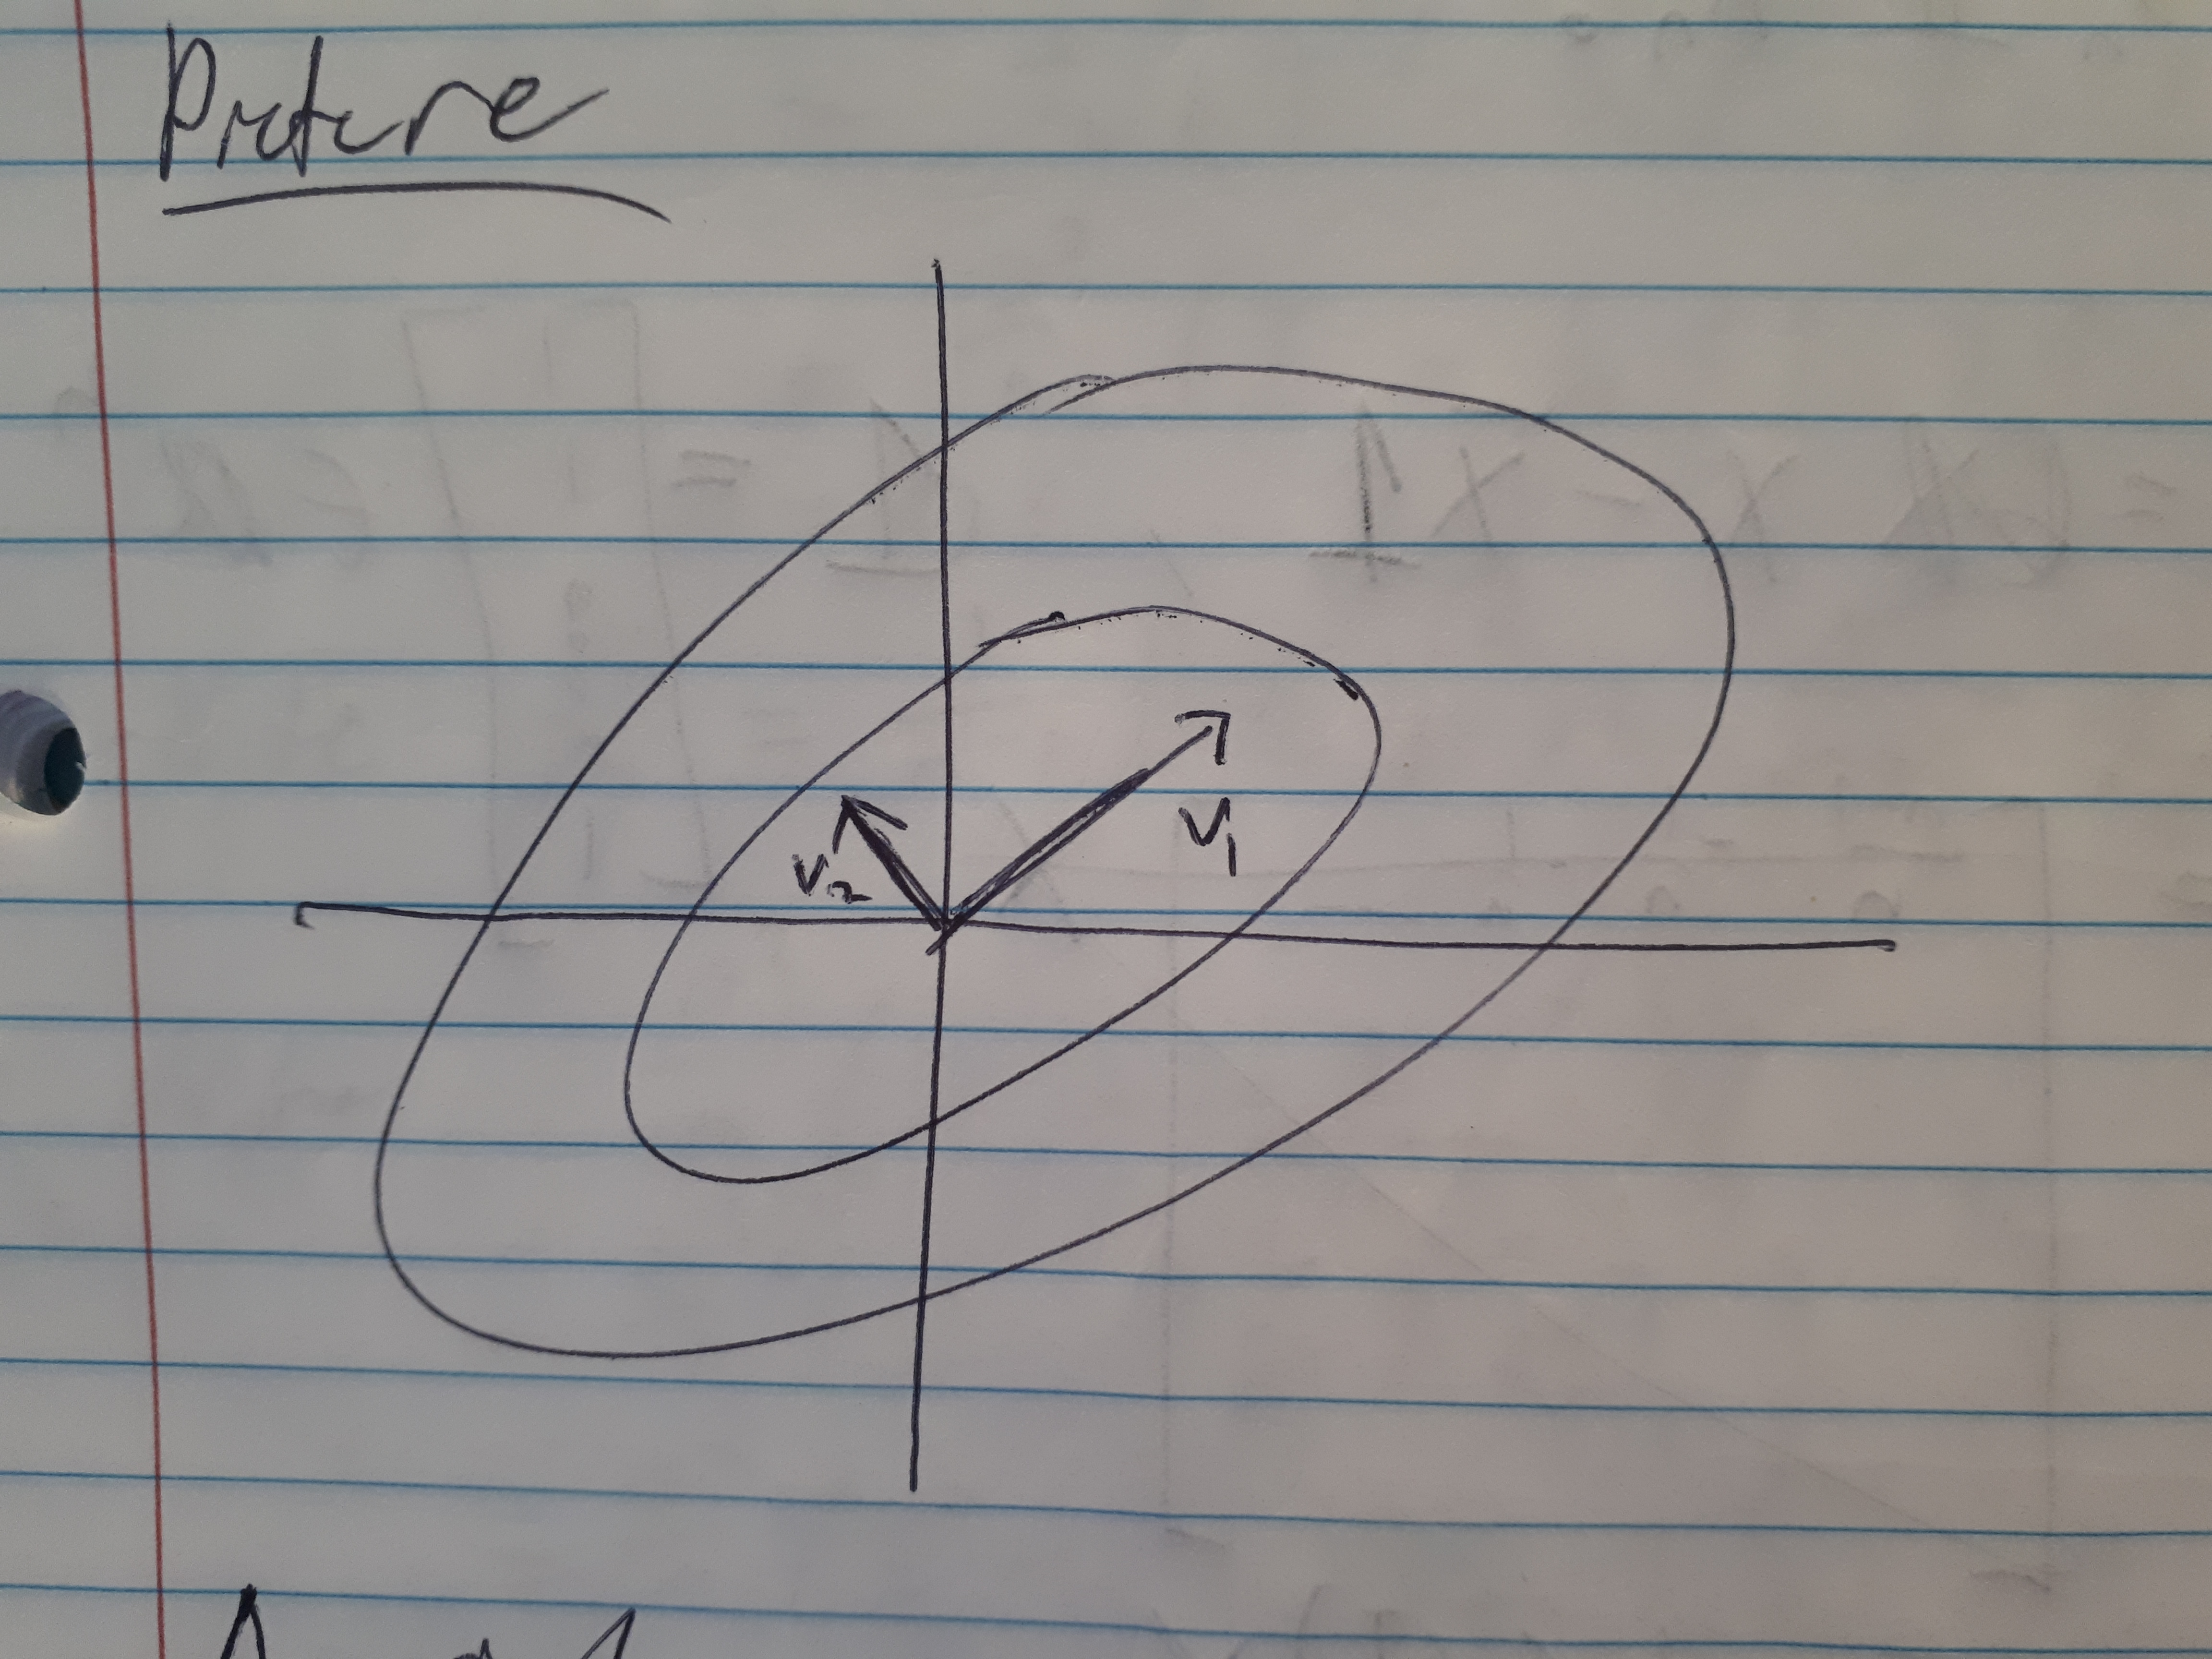
\includegraphics[width = \textwidth/2]{09_30_P01.jpg}
    
\end{center}
\subsection{Hypothesis tests and the T distribution}
Suppose we have data $X_i$ from some process and we want to test
\[\E[X_i] = 0 \text{ vs } \E[X_i] \neq 0. \]
We form a null hypothesis $H_0 : \{X_i \iid N(0,\sigma^2)\}$ where $\sigma^2$ is unknown. If we assume that $H_0$ is true, then 
\[\bar{X}_n := \frac{1}{n}\sum_{i=1}^n X_i \sim N(0, \sigma^2/n), \]
\[S_n^2 := \frac{1}{n-1}\sum_{i=1}^n (X_i-\bar{X}_n)^2 \sim \frac{\sigma^2}{n-1}\chi^2_{n-1}, \]
and $S_n^2 \ind \bar{X}_n$. 
\begin{proof}
    Let $Z = X - \bar{X}_n \one$, where 
    \[\one = \begin{bmatrix}
        1\\ \vdots \\ 1
    \end{bmatrix} \in \R^n.\]
    We can rewrite this as $Z = X - \bar{X}_n\one = (I-\frac{1}{n}\one\one^T)X$. Set $\Pi = I-\frac{1}{n}\one\one^T$, then $\Pi^2 = \Pi$ so $\Pi$ is a projection. In fact $\Pi$ projects onto the orthogonal complement of $\one$. Also note that $\bar{X}_n = \frac{1}{n}\one^T X$. Thus 
    \[\begin{bmatrix}
        \bar{X}_n\\ Z
    \end{bmatrix}\sim \Na\left(\begin{bmatrix}
        0\\0
    \end{bmatrix}, \begin{bmatrix}
        \frac{\sigma^2}{n}&\_ \\
        \_& \sigma^2\left(I - \frac{1}{n}\one\one^T\right)
    \end{bmatrix}\right). \]
    We wish to fill in the blanks in the above covariance matrix. In particular we want to show that they are zero. Note that these blanks equal
    \begin{IEEEeqnarray*}{rCl}
        \E[Z\bar{X}_n] &=&\frac{1}{n}\E\left[\left(I - \frac{1}{n}\one\one^T\right)XX^T\one\right]\\
        &=&\frac{1}{n}\left(I-\frac{1}{n}\one\one^T\right)\E[XX^T]\one\\
        &=&\frac{1}{n}\left(I-\frac{1}{n}\one\one^T\right)\sigma^2 I\one\\
        &=&\frac{\sigma^2}{n}\left(I-\frac{1}{n}\one\one^T\right)\one\\
        &=& \frac{\sigma^2}{n}\left(\one - \frac{1}{n}\one \norm{\one}_2^2\right)\\
        &=&\frac{\sigma^2}{n}\left(\one - \one\right)\\
        &=&0.
    \end{IEEEeqnarray*}
    Thus $\bar{X}_n \ind Z$ and so $\bar{X}_n \ind S_n^2$ and also  $S_n^2 = \frac{1}{n-1}\norm{Z}^2_2 \sim \frac{\sigma^2}{n-1}\chi_{n-1}^2$.
\end{proof}
\begin{defn}
Let $X \sim N(0,1)$ and $S^2 \sim \chi_d^2$ with $X \ind S^2$, then the ratio 
\[\frac{X}{\sqrt{\frac{1}{d}S^2}}, \]
has a T-distribution (also called a Student's t-distribution) with $d$ d.o.f.
\end{defn}
Recall our hypothesis $H_0 : \{X_i \sim N(0,\sigma^2)\}$. Under this hypothesis the statistic 
\[T_n := \frac{\bar{X}_n}{\sqrt{\frac{1}{n-1}S_n^2}} \sim T_{n-1}. \]
That is our statistic has a $T$ distribution with $(n-1)$ degrees of freedom regardless of what $\sigma^2$ is. We next calculate our $p$ value which is the probability under the null of observing data as ``weird'' as what we observed (where ``weird'' is something subjective that can vary). We then check if our $p$ value is below some predetermined threshold $\al$. 

In the one-sided T-test we reject if 
\[\Pa(T_{n-1} \ge t_n) \le \al, \]
where $\al$ is the level of our test, $T_{n-1}$ has a $T$ distribution with $(n-1)$ d.o.f. and $t_n$ is our statistic calculated from the data. In this case observed data is ``weird'' if it is very big and positive.

In the two-side T-test we reject if
\[\Pa(\abs{T_{n-1}}\ge \abs{t_n}) \le \al, \]
where $\al, T_{n-1}$ and $t_n$ are as above. In this case our data is ``weird'' if it is very big and either positive or negative. We could also have some other meaning of ``weird''. Note the following important points:
\begin{itemize}
    \item $p$-values say \emph{nothing} about the truth.
    \item They only say something about what \emph{isn't} true.
    \item The $t$-test is fairly robust to non-normal data.
    \item The $t$-test is not robust to the case when the variables are dependent.
\end{itemize}
\subsection{F-distributions}
let $Z_1 \sim \chi_d$ and $Z_2 \sim \chi_n$ with $Z_1 \ind Z_2$, then the ratio
\[\frac{\frac{1}{d}Z_1}{\frac{1}{n}Z_2}, \]
has Fisher's $F$-distribution with $(d,n)$ d.o.f. We will sometimes say $d$ d.o.f on the top and $n$ d.o.f on the bottom. We expect 
\[\frac{\frac{1}{d}Z_1}{\frac{1}{n}Z_2}, \]
to be close to 1.

\section{Least squares and linear models}
Starting assumptions 
\[Y=X\beta + \varepsilon, \]
where $X \in \R^{n \times d}$, $\beta \in \R^d$ and $\varepsilon \in \R^n$. Our assumptions on $\varepsilon$ will vary. We will always assume (a) but sometimes we will make stronger assumptions like (b) and (c)
\begin{enumerate}
    \item $\E[\varepsilon] = 0$ and $\text{cov}(\varepsilon) = \sigma^2I_n$,
    \item $\varepsilon_i \iid (0,\sigma^2)$,
    \item $\varepsilon_i \iid \Na(0,\sigma^2)$.
\end{enumerate}
We will represent $X$ in the following way
\[X = \begin{bmatrix}
    x_1^T\\ \vdots \\ x_n^T
\end{bmatrix}, \]
and usually we will have $X_{i,1} = 1$ for all $i$ which means our model has an intercept.

We saw previously that our estimator is given by 
\[\wh{\beta} = \amin_b \frac{1}{2}\norm{Xb - Y}_2^2. \]
Recall that this is equivalent to $\wh{\beta}$ satisfying the normal equations. That is we want
\[ X^TX\wh{\beta} = X^TY.\]
(Typically $X$ will have rank $d$ (full rank) and then $\wh{\beta} = (X^TX)^{-1}X^TY$.)
\subsection{Geometric picture}
$\Ma = \{Xb : b \in \R^d\}$ is our model space. $H = X(X^TX)^{-1}X^T$ is the matrix that projects onto $\Ma$ and we call it the hat matrix. 

Define the predicted values \[\wh{Y} = X\wh{\beta} = X(X^TX)^{-1}X^T Y = HY.\] And the residuals/estimated error
\[\wh{\varepsilon}=Y-\wh{Y} = (I-H)Y.\]
We then have $\varepsilon \perp \Ma$ ($\varepsilon$ is orthogonal to $\Ma$, see picture). 
\begin{center}
    
    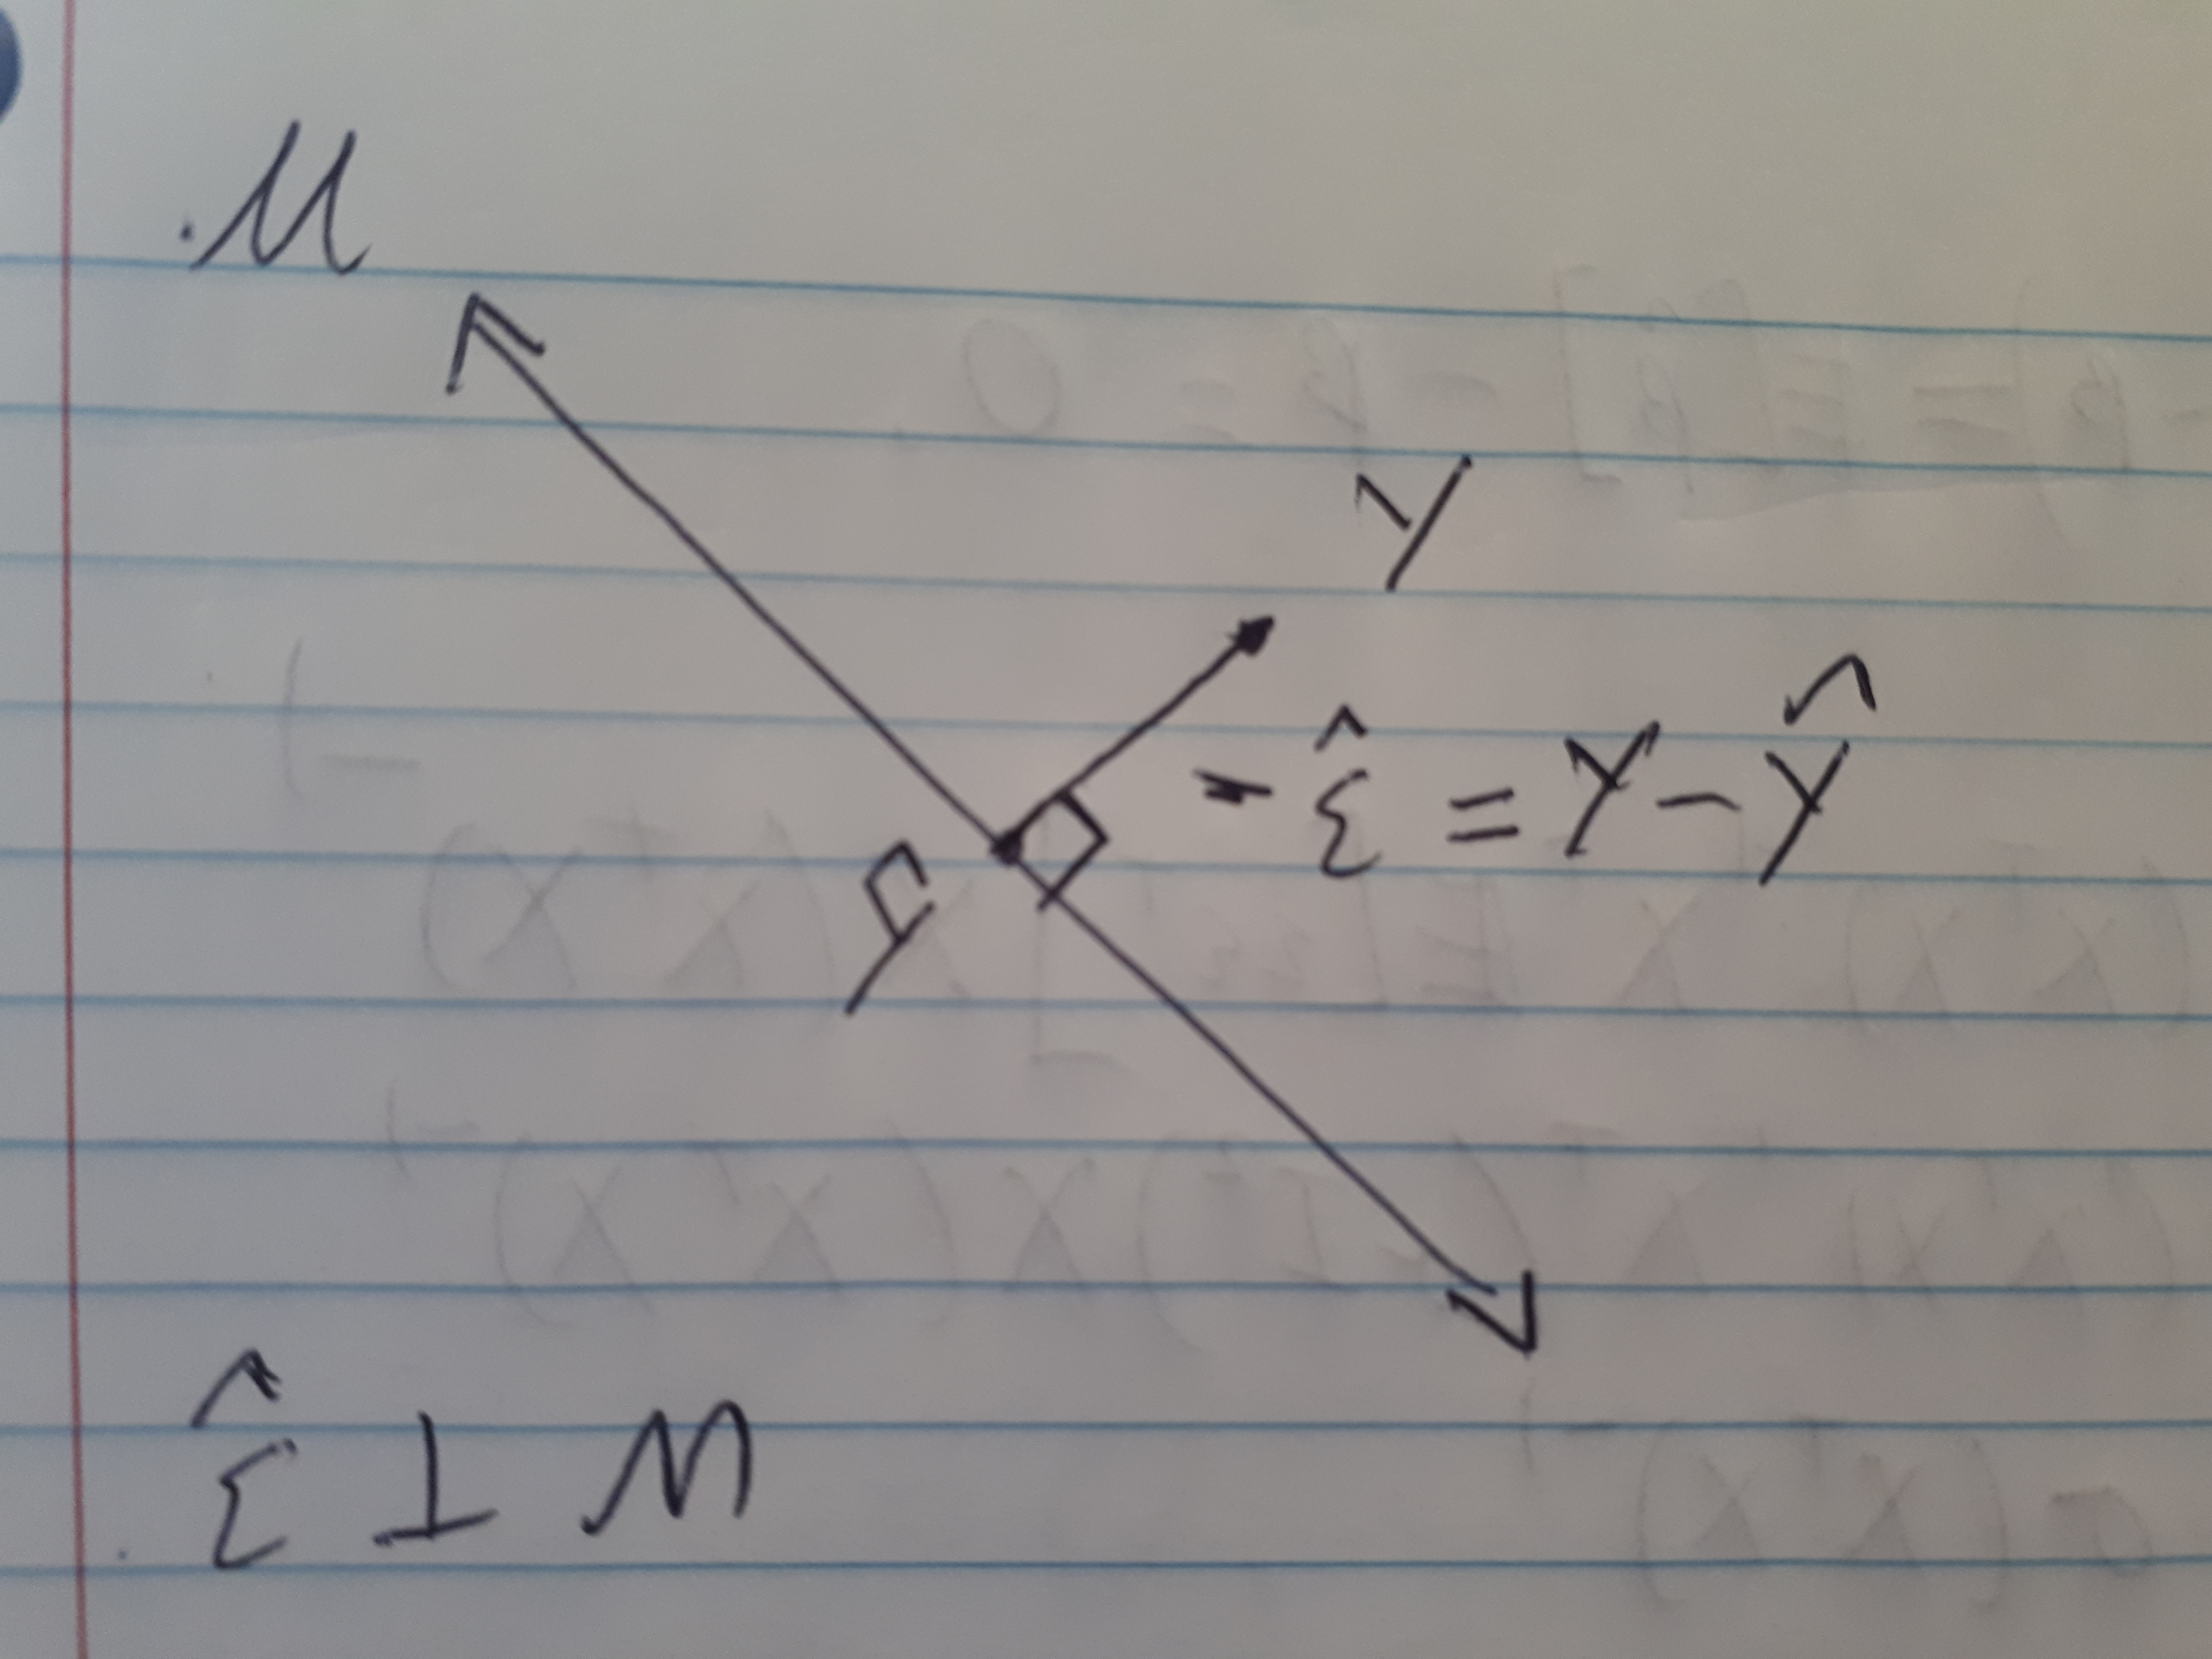
\includegraphics[width = \textwidth/2]{09_30_P02.jpg}
    
\end{center}
We can see this by using the normal equations which state that $X^TX\wh{\beta}-X^TY = 0$. Thus 
\[X^T\wh{\varepsilon}= X^T(\wh{Y}-Y) = X^T(X\wh{\beta}-Y)= X^TX\wh{\beta}-X^TY =0. \]

\subsection{Distributional results}
Can we get distributional results from this picture?
\begin{thrm}
Assume that $X$ has rank $d \le n$ and that $\E[\varepsilon]=0$ and $\text{cov}(\varepsilon) = \sigma^2I$ (this was our weakest assumption on $\varepsilon$), then
\begin{enumerate}
    \item $\E[\wh{\beta}] = \beta$ (that is $\wh{\beta}$ is unbiased for $\beta$).
    \item $\text{cov}(\wh{\beta}) = \sigma^2 (X^TX)^{-1}$.
\end{enumerate}
\end{thrm}
\begin{proof}
    \begin{enumerate}
        \item $\E[\wh{\beta}] = (X^TX)^{-1}X^T\E[Y] =X^TX)^{-1}X^TX\beta = \beta$.
        \item Note that $\E[\wh{\beta} - \beta] = \E[\wh{\beta}]-\beta = 0$. Thus 
        \begin{IEEEeqnarray*}{rCl+x+}
            \text{cov}(\wh{\beta})&=&(X^TX)^{-1}X^T\E[\varepsilon\varepsilon^T]X(X^TX)^{-1}\\
            &=&(X^TX)^{-1}X^T\sigma^2 I_nX(X^TX)^{-1}\\
            &=&\sigma^2 (X^TX)^{-1}.&\qedhere
        \end{IEEEeqnarray*}
    \end{enumerate}
\end{proof}
If we use our strongest assumptions we have
\begin{thrm}\emph{[Important -  will be used a lot]}
    Assume $X$ has rank $d$ and $\varepsilon \sim \Na(0,\sigma^2 I)$, then
    \begin{enumerate}
        \item $\wh{\beta} \sim \Na(\beta,\sigma^2(X^TX)^{-1})$.
        \item $\wh{Y} = HY \sim \Na(X\beta, \sigma^2 H)$.
        \item $\wh{\varepsilon} = (I-H)Y \sim \Na(0, \sigma^2(I-H))$.
    \end{enumerate}
    And $\wh{\varepsilon} \ind (\wh{\beta}, \wh{Y})$.
\end{thrm}
\begin{proof}
    \begin{enumerate}
        \item We know $\wh{\beta} - \beta = (X^TX)^{-1}X^T\varepsilon$ and so $\wh{\beta} - \beta \sim \Na(0, \sigma^2(X^TX)^{-1})$ from before.
        \item $HY = H(X\beta+\varepsilon)=X\beta+H\varepsilon$ and $H^2 = H$. Thus $HY  \sim \Na(X\beta, \sigma^2 H)$.
        \item $(I-H)Y = (I-H)(X\beta + \varepsilon) = (I-H)\varepsilon$, since $I-H$ is a projection we have $(I-H)Y \sim \Na(0, \sigma^2(I-H))$.
    \end{enumerate}
    For independence note that
    \begin{IEEEeqnarray*}{rCl}
        \text{cov}(\wh{\varepsilon}, \wh{Y}) &=&\E[(I-H)Y(H(Y-\E Y))^T]\\
        &=&(I-H)\E[Y(Y-\E  Y)^T]H\\
        &=&(I-H)\sigma^2IH\\
        &=&0.
    \end{IEEEeqnarray*}
    Thus $\wh{\varepsilon} \ind \wh{Y}$ and the proof that $\wh{\varepsilon} \ind \wh{\beta}$ is similar.
\end{proof}

\end{document}